%&pdfLaTeX
% !TEX encoding = UTF-8 Unicode
\documentclass{article}
\usepackage{ifxetex}
\ifxetex
\usepackage{fontspec}
\setmainfont[Mapping=tex-text]{STIXGeneral}
\else
\usepackage[T1]{fontenc}
\usepackage[utf8]{inputenc}
\fi
\usepackage{textcomp}

\usepackage{graphicx}
\usepackage{array}
\usepackage{ulem}
\usepackage{amssymb}
\usepackage{fancyhdr}
\renewcommand{\headrulewidth}{0pt}
\renewcommand{\footrulewidth}{0pt}
\usepackage{color}

\definecolor{color02}{rgb}{0.25,0.25,0.25}
\definecolor{color03}{rgb}{0.00,0.00,0.04}
\definecolor{color04}{rgb}{1.00,1.00,1.00}
\definecolor{color09}{rgb}{0.17,0.08,0.18}

\begin{document}

\begin{center}
{\Huge{}{\color{color04} CloudFerry}}
\end{center}

\vspace{2pt}
\baselineskip=12pt
%%\begin{figure}[htbp]
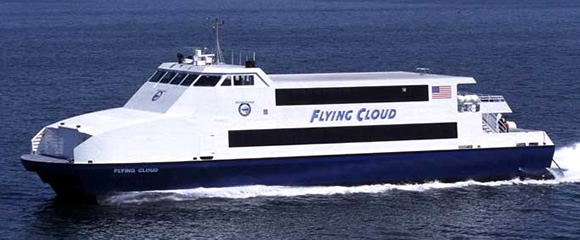
\includegraphics[width=250, height=105, keepaspectratio=true]{images/CloudFerry_Brochure-fig001.jpg}
%%\caption{This should be the caption for \texttt{CloudFerry\_Brochure-fig001.jpg}.}
%%\end{figure}

\vspace{24pt}
\hline
{\Huge{}{\color{color04} Cloud Resource Migration Tool}}\linebreak{}
{\Huge{}{\color{color04} Feature Overview}}
\hline

\vspace{36pt}
\section*{{\Huge{}{\color{color04} Overview}}}

\vspace{2pt}
%%\begin{figure}[htbp]

\includegraphics[width=254pt, height=300pt, keepaspectratio=true]{images/CloudFerry_Brochure-fig002.png}
%%\caption{This should be the caption for \texttt{CloudFerry\_Brochure-fig002.png}.}
%%\end{figure}

\vspace{2pt}
{\large{}{\color{color03} \textbf{What is it?}}}

\vspace{2pt}
{\color{color03} Quite simply, CloudFerry is an open-source tool for resource and 
workload migration between OpenStack clouds. A ``workload'' is a virtual machine 
and all the resources that were used to create it. }

\vspace{2pt}
{\large{}{\color{color03} \textbf{Why?}}}

\vspace{2pt}
{\color{color03} Within an OpenStack cloud environment there may be many Tenants. 
Within a tenant there are many workloads which are composed from resources like 
images, flavors, block storage volumes, etc... Occasionally Cloud operators will 
need to move Cloud resident resources and workloads from one environment to another. 
Doing so manually is a tedious and risky process which has many steps, challenges 
and pitfalls. }

\vspace{2pt}
{\color{color03} CloudFerry provides a source of automation for the task of resource 
and workload migration between OpenStack Clouds that makes a virtue of removing 
most of the risk and speeding the process tremendously; just like automation is 
supposed to do. CloudFerry comes with useful pre-fabricated configurations but 
is also highly configurable. Users can use the with minimal customization or they 
can go completely custom to meet their requirements. }

\section*{{\Huge{}{\color{color04} Features}}}

{\large{}{\color{color03} \textbf{Condensation}}}

\vspace{2pt}
{\color{color03} Condensation is simply creating a scenario file that will be used 
during the Evacuation phase. It is done within a single cloud and is meant to figure 
out how to minimize the number of physical nodes handling the total workload. Condensation 
is a tricky and slow task to do manually but is fairly simple to do with CloudFerry. 
Much of the difficulty of doing things manually comes from the Knapsack Problem 
which can be solved with a little math but much like all things that can be solved 
with math, it's easier and better to let the machines get on with the adding up 
and leave the contemplation of larger issues to the working thinkers.}

\vspace{2pt}
\begin{center}
%%\begin{figure}[htbp]
\includegraphics[width=137pt, height=145pt, keepaspectratio=true]{images/CloudFerry_Brochure-fig003.wmf}
%%\caption{This should be the caption for \texttt{CloudFerry\_Brochure-fig003.wmf}.}
%%\end{figure}

\end{center}

\vspace{2pt}
{\color{color03} \textbf{The Knapsack Problem}}

\vspace{2pt}
{\color{color02} The knapsack problem simply stated is: }{\color{color02} \textit{Given 
a set of items, each with a mass and a value, determine the number of each item 
to include in a collection so that the total weight is less than or equal to a 
given limit and the total value is as large as possible. }}

\vspace{2pt}
{\color{color02} It derives its name from the problem faced by someone who is constrained 
by a fixed-size }{\color{color02} \emph{knapsack}}{\color{color02}  and must fill 
it with the most valuable items. There are well known mathematical and algorithmic 
solutions to the problem. Given the }

\vspace{2pt}
\begin{center}
%%\begin{figure}[htbp]
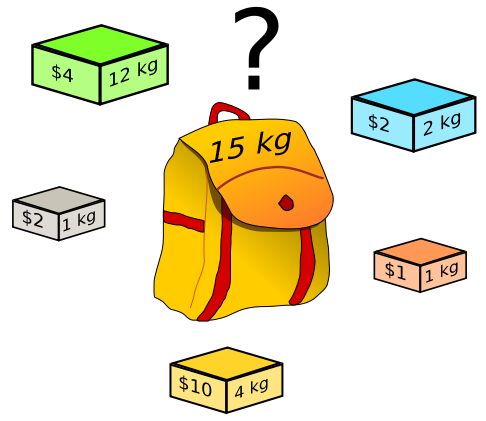
\includegraphics[width=186pt, height=161pt, keepaspectratio=true]{images/CloudFerry_Brochure-fig004.png}
%%\caption{This should be the caption for \texttt{CloudFerry\_Brochure-fig004.png}.}
%%\end{figure}

\end{center}

\vspace{4pt}
\baselineskip=12pt

{\color{color03} When the condensation feature is executed it will not make any 
changes to the cloud. It will simply output a file which will define the sequence 
and placement of VM's that the Evacuation phase will execute against. Evacuation 
is run separately from condensation making the Condensation operation purely informative 
if not followed up by Evacuation. The scenario file that is generated can be modified 
before Evacuation is run in order to accommodate specific needs or used as is.}

\vspace{30pt}
{\large{}{\color{color03} \textbf{Evacuation}}}

\vspace{2pt}
{\color{color03} Evacuation within the context of CloudFerry is the stage where 
the scenario file created by the Condensation phase is used as a control input 
to actually move workloads around within a single cloud to minimize the number 
of physical nodes in use. The net result is all the servers that have any load 
on them at all are likely to have quite a lot of load on them until environment 
is rebalanced or migrated (some rebalancing is a by-product of migrating). Once 
Evacuation is undertaken it would be wise to move forward through to migration 
or to manually rebalance workload distribution as quickly as practicable since 
the failure cost of any one physical node going down is larger than it was before 
Evacuation was run.}

\vspace{2pt}
{\color{color03} If, for example, you need to be able to spawn a series of big 
VM's but no single node has enough spare resources to contain one then you could 
use the Condensation and Evacuation features as a set of tools to move things around 
to a maximal load:node ratio thereby freeing up the contiguous resources you need 
to spawn that set of large VM's. That is of course only one example; and a very 
primitive one at that, of a use case in an infinite world of possibilities and 
motivations. The primary purpose of the Condensation and Evacuation features is 
to allow cloud operators to clear physical nodes so that they can be moved to a 
new cloud and the resources and workloads migrated to that new cloud. It is not 
meant for finely managing the node:workload layout within any single cloud. }

\vspace{2pt}
{\color{color03} Evacuation can be configured to deal with the whole of the set 
of nodes within a cloud or restricted to any arbitrary subset of nodes through 
the use of filter files and the modification of the scenario file that is outputted 
as part of the Condensation run. Evacuation allows two possible back-ends to be 
used - cobalt and nova live-migrate. }

\vspace{2pt}
\begin{center}
%%\begin{figure}[htbp]
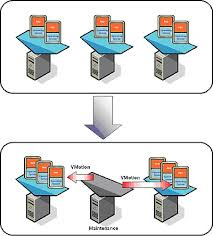
\includegraphics[width=220, height=242pt, keepaspectratio=true]{images/CloudFerry_Brochure-fig005.jpg}
%%\caption{This should be the caption for \texttt{CloudFerry\_Brochure-fig005.jpg}.}
%%\end{figure}

\end{center}

\vspace{54pt}
\baselineskip=12pt

{\large{}{\color{color03} \textbf{Migration}}}

\begin{center}
%%\begin{figure}[htbp]
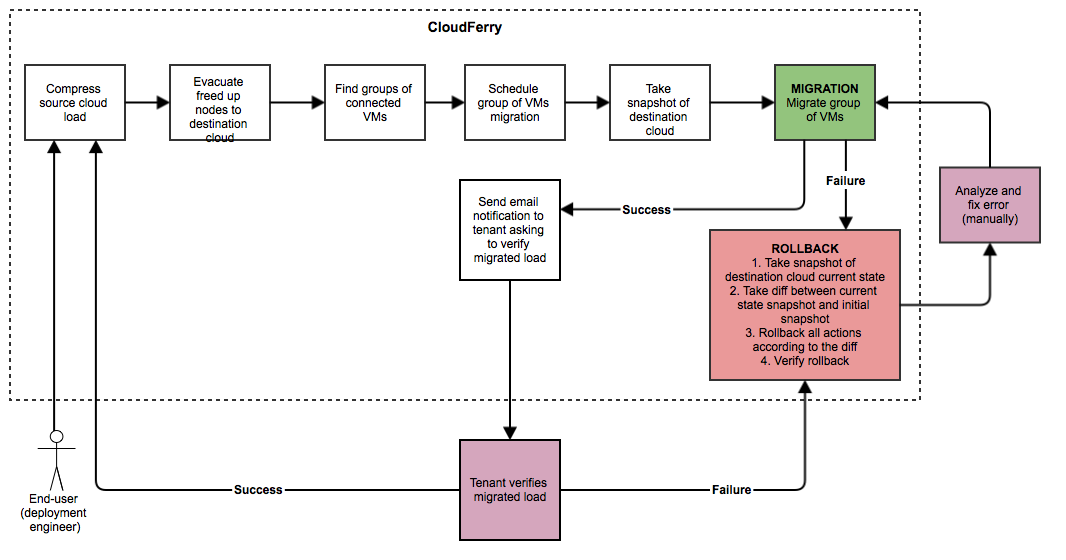
\includegraphics[width=285pt, height=150, keepaspectratio=true]{images/CloudFerry_Brochure-fig006.png}
%%\caption{This should be the caption for \texttt{CloudFerry\_Brochure-fig006.png}.}
%%\end{figure}

\vspace{2pt}
{\small{}{\color{color09} \textit{Figure 1: CloudFerry Migration Process Cycle}}}
\end{center}

\vspace{2pt}
\baselineskip=12pt

{\color{color03} Migration in the context of CloudFerry focuses on whole Tenants 
rather than Tenant resources. Migration refers to moving an entire tenant from 
one OpenStack Cloud to another. That includes workloads as well as resources. It 
is the last stage in the process and uses the work done during Condensation and 
Evacuation. Many of the same challenges encountered with Evacuation activities 
are found when migrating as well as many others specific to migration. The difficulty, 
time involved and risk involved in manually migrating tenants is significant and 
most organizations simply cannot tolerate that level of risk. CloudFerry minimizes 
the risk partly by providing a scenario and sticking to it and largely by keeping 
necessary human actions to a minimum.}

\begin{center}
%%\begin{figure}[htbp]

\includegraphics[width=180pt, height=150pt, keepaspectratio=true]{images/CloudFerry_Brochure-fig007.png}
%%\caption{This should be the caption for \texttt{CloudFerry\_Brochure-fig007.png}.}
%%\end{figure}

\end{center}

\vspace{24pt}
\baselineskip=12pt

{\color{color03} Thanks to the use of layered configuration specificity CloudFerry 
is highly flexible and can accommodate very complex migration requirements and 
constraints. It should be noted that CloudFerry is a tool, not a magic wand. Cloud 
operators who are undertaking migration activities will want to make things as 
easy on themselves as possible at each phase of the project. Thorough planning 
is still necessary even with the best tools available.}

\vspace{30pt}
{\large{}{\color{color03} \textbf{Nominal Use Case}}}

\vspace{2pt}
{\color{color03} An enterprise has an existing OpenStack cloud running an older 
release and wants to upgrade. CloudFerry provides the Condensation, Evacuation 
and Migration functionality making this process less confusing, less error prone 
and massively faster than any manual means.}

\vspace{24pt}
\begin{center}
%%\begin{figure}[htbp]

\includegraphics[width=235pt, height=169pt, keepaspectratio=true]{images/CloudFerry_Brochure-fig008.jpg}
%%\caption{This should be the caption for \texttt{CloudFerry\_Brochure-fig008.jpg}.}
%%\end{figure}

\end{center}

\vspace{24pt}
\baselineskip=12pt

{\color{color03} Since OpenStack doesn't provide a direct software upgrade path 
the Cloud operator will start by building a small OpenStack cloud with enough hardware 
to take the first few tenants with the latest OpenStack release. They then run 
CloudFerry Condensation to determine the number of physical nodes that can be freed 
up and moved to the destination cloud. They then run Evacuation to get the legacy 
cloud workloads onto as few nodes as possible. Once the source cloud has been compacted 
the Cloud operator can move the freed up physical nodes to the new cloud and gradually 
migrate workloads into the new cloud to use the migrated hardware. }

\vspace{2pt}
{\color{color03} Migrations are done tenant-by-tenant which allows a measure of 
granularity, control and flexibility making the process massively easier than it 
would be to do manually. It also means that you don't use CloudFerry to move a 
single instance from Cloud-A to Cloud-B. }

\vspace{2pt}
{\color{color03} If a particular server or set of servers needs to be freed up 
for any reason before some other set then an Evacuation can be performed against 
those specific servers or filters can be used to set the order of operations or 
the operator can manually migrate the instances from those nodes and run Condensation 
after that. }

\vspace{2pt}
{\color{color03} Now that resources are in place to take the first wave of workload, 
migration can be undertaken. A tenant is chosen for migration and moved to the 
new OpenStack Cloud using CloudFerry. As hardware is freed up it can be moved to 
the destination cloud. It may become necessary, depending on how much hardware 
was provisioned for the destination cloud in the first place, to run multiple Condensation 
and/or Evacuation processes along the way. Once all tenants have been migrated 
the source cloud can be dismantled and its remaining resources added to the destination 
cloud. Project complete!}

\vspace{22pt}
{\large{}{\color{color03} \textbf{Pre-Migration Considerations:}}}

\vspace{2pt}
{\large{}{\color{color03} \textbf{Application Fault Tolerance:}}}

\vspace{2pt}
{\color{color03} Properly designed cloud capable applications are distributed across 
many availability zones and should be able to tolerate bringing down of a single 
availability zone without substantially degrading performance or functionality. 
CloudFerry operates only within a single availability zone which means that while 
all of the availability zones aren't running, the application remains available 
as far as the consumer of that application knows. }

\vspace{2pt}
{\large{}{\color{color03} \textbf{Requirements:}}}

$\Psi$ {\color{color03} Connection to source and destination clouds through external(public) 
network from host with CloudFerry.}

$\Psi$ {\color{color03} Valid private ssh-key for both clouds which will be used 
by CloudFerry for data transferring.}

$\Psi$ {\color{color03} Admin keystone access (typically admin access point lives 
on 35357 port).}

$\Psi$ {\color{color03} sudo/root access on compute and controller nodes.}

$\Psi$ {\color{color03} Openstack MySQL DB write access.}

$\Psi$ {\color{color03} Credentials of global cloud admin for both clouds.}

$\Psi$ {\color{color03} All the Python requirements are listed in the package in 
requirements.txt.}

{\large{}{\color{color03} \textbf{Other Important Factors: }}}

\vspace{2pt}
\parindent=3pt
$\Psi$ {\color{color03} The amount of time it takes to migrate a tenant will depend 
completely upon the speed of the network.  }

$\Psi$ {\color{color03} Condensation of VM's is fast. Condensation of Software 
Defined Networks can be exceptionally slow due to limitations of the Neutron API. 
}

$\Psi$ {\color{color03} CloudFerry configuration can be described as non-trivial. 
Just like any highly configurable system. It is advised that users take a little 
while to get to know CloudFerry before attempting to use it on a production environment. 
 }

$\Psi$ {\color{color03} CloudFerry works via SSH/SCP, MySQL transactions and OpenStack 
API calls.  }

$\Psi$ {\color{color03} Considerable knowledge of OpenStack is a requirement for 
successful use of CloudFerry.}

\vspace{2pt}
\parindent=0pt
{\large{}{\color{color03} \textbf{Live Migration:}}}

\vspace{2pt}
{\color{color03} Live Migration is tiny bit of a misnomer. When you migrate tenants 
between clouds there will be a period of unavailability for the workloads and resources 
being moved, however brief. Live migration uses block migration which alleviates 
the need to take snapshots. That means the instance doesn't need to quiesce to 
migrate and can stay up and running.  }

\vspace{2pt}
{\large{}{\color{color03} \textbf{Cold Migration:}}}

\vspace{2pt}
{\color{color03} Cold migration is a pretty accurate term but may give the impression 
that things need to be dark. This is a mode where the tenant environment can be 
shut down but does not need to. In cold migration the same VM instance will be 
booted on the destination cloud that was on the source cloud. There will be downtime 
during cold migration as ephemeral storage is copied over to the destination cloud. 
When you use the cold migration scenario as it comes,\label{HGoBack} CloudFerry 
will pause each instance (virtual machine), take a snapshot of the instance, copy 
the snapshot to the destination cloud along with taking care of provisioning and 
copying any resources that the instance uses. It then brings the instance back 
online. The automated verifications are currently relatively limited and a manual 
verification should be completed before production traffic is allowed to be directed 
back to the migrated tenant.}

\newpage

\end{document}
